
% Default to the notebook output style

    


% Inherit from the specified cell style.




    
\documentclass[11pt]{article}

    
    
    \usepackage[T1]{fontenc}
    % Nicer default font (+ math font) than Computer Modern for most use cases
    \usepackage{mathpazo}

    % Basic figure setup, for now with no caption control since it's done
    % automatically by Pandoc (which extracts ![](path) syntax from Markdown).
    \usepackage{graphicx}
    % We will generate all images so they have a width \maxwidth. This means
    % that they will get their normal width if they fit onto the page, but
    % are scaled down if they would overflow the margins.
    \makeatletter
    \def\maxwidth{\ifdim\Gin@nat@width>\linewidth\linewidth
    \else\Gin@nat@width\fi}
    \makeatother
    \let\Oldincludegraphics\includegraphics
    % Set max figure width to be 80% of text width, for now hardcoded.
    \renewcommand{\includegraphics}[1]{\Oldincludegraphics[width=.8\maxwidth]{#1}}
    % Ensure that by default, figures have no caption (until we provide a
    % proper Figure object with a Caption API and a way to capture that
    % in the conversion process - todo).
    \usepackage{caption}
    \DeclareCaptionLabelFormat{nolabel}{}
    \captionsetup{labelformat=nolabel}

    \usepackage{adjustbox} % Used to constrain images to a maximum size 
    \usepackage{xcolor} % Allow colors to be defined
    \usepackage{enumerate} % Needed for markdown enumerations to work
    \usepackage{geometry} % Used to adjust the document margins
    \usepackage{amsmath} % Equations
    \usepackage{amssymb} % Equations
    \usepackage{textcomp} % defines textquotesingle
    % Hack from http://tex.stackexchange.com/a/47451/13684:
    \AtBeginDocument{%
        \def\PYZsq{\textquotesingle}% Upright quotes in Pygmentized code
    }
    \usepackage{upquote} % Upright quotes for verbatim code
    \usepackage{eurosym} % defines \euro
    \usepackage[mathletters]{ucs} % Extended unicode (utf-8) support
    \usepackage[utf8x]{inputenc} % Allow utf-8 characters in the tex document
    \usepackage{fancyvrb} % verbatim replacement that allows latex
    \usepackage{grffile} % extends the file name processing of package graphics 
                         % to support a larger range 
    % The hyperref package gives us a pdf with properly built
    % internal navigation ('pdf bookmarks' for the table of contents,
    % internal cross-reference links, web links for URLs, etc.)
    \usepackage{hyperref}
    \usepackage{longtable} % longtable support required by pandoc >1.10
    \usepackage{booktabs}  % table support for pandoc > 1.12.2
    \usepackage[inline]{enumitem} % IRkernel/repr support (it uses the enumerate* environment)
    \usepackage[normalem]{ulem} % ulem is needed to support strikethroughs (\sout)
                                % normalem makes italics be italics, not underlines
    

    
    
    % Colors for the hyperref package
    \definecolor{urlcolor}{rgb}{0,.145,.698}
    \definecolor{linkcolor}{rgb}{.71,0.21,0.01}
    \definecolor{citecolor}{rgb}{.12,.54,.11}

    % ANSI colors
    \definecolor{ansi-black}{HTML}{3E424D}
    \definecolor{ansi-black-intense}{HTML}{282C36}
    \definecolor{ansi-red}{HTML}{E75C58}
    \definecolor{ansi-red-intense}{HTML}{B22B31}
    \definecolor{ansi-green}{HTML}{00A250}
    \definecolor{ansi-green-intense}{HTML}{007427}
    \definecolor{ansi-yellow}{HTML}{DDB62B}
    \definecolor{ansi-yellow-intense}{HTML}{B27D12}
    \definecolor{ansi-blue}{HTML}{208FFB}
    \definecolor{ansi-blue-intense}{HTML}{0065CA}
    \definecolor{ansi-magenta}{HTML}{D160C4}
    \definecolor{ansi-magenta-intense}{HTML}{A03196}
    \definecolor{ansi-cyan}{HTML}{60C6C8}
    \definecolor{ansi-cyan-intense}{HTML}{258F8F}
    \definecolor{ansi-white}{HTML}{C5C1B4}
    \definecolor{ansi-white-intense}{HTML}{A1A6B2}

    % commands and environments needed by pandoc snippets
    % extracted from the output of `pandoc -s`
    \providecommand{\tightlist}{%
      \setlength{\itemsep}{0pt}\setlength{\parskip}{0pt}}
    \DefineVerbatimEnvironment{Highlighting}{Verbatim}{commandchars=\\\{\}}
    % Add ',fontsize=\small' for more characters per line
    \newenvironment{Shaded}{}{}
    \newcommand{\KeywordTok}[1]{\textcolor[rgb]{0.00,0.44,0.13}{\textbf{{#1}}}}
    \newcommand{\DataTypeTok}[1]{\textcolor[rgb]{0.56,0.13,0.00}{{#1}}}
    \newcommand{\DecValTok}[1]{\textcolor[rgb]{0.25,0.63,0.44}{{#1}}}
    \newcommand{\BaseNTok}[1]{\textcolor[rgb]{0.25,0.63,0.44}{{#1}}}
    \newcommand{\FloatTok}[1]{\textcolor[rgb]{0.25,0.63,0.44}{{#1}}}
    \newcommand{\CharTok}[1]{\textcolor[rgb]{0.25,0.44,0.63}{{#1}}}
    \newcommand{\StringTok}[1]{\textcolor[rgb]{0.25,0.44,0.63}{{#1}}}
    \newcommand{\CommentTok}[1]{\textcolor[rgb]{0.38,0.63,0.69}{\textit{{#1}}}}
    \newcommand{\OtherTok}[1]{\textcolor[rgb]{0.00,0.44,0.13}{{#1}}}
    \newcommand{\AlertTok}[1]{\textcolor[rgb]{1.00,0.00,0.00}{\textbf{{#1}}}}
    \newcommand{\FunctionTok}[1]{\textcolor[rgb]{0.02,0.16,0.49}{{#1}}}
    \newcommand{\RegionMarkerTok}[1]{{#1}}
    \newcommand{\ErrorTok}[1]{\textcolor[rgb]{1.00,0.00,0.00}{\textbf{{#1}}}}
    \newcommand{\NormalTok}[1]{{#1}}
    
    % Additional commands for more recent versions of Pandoc
    \newcommand{\ConstantTok}[1]{\textcolor[rgb]{0.53,0.00,0.00}{{#1}}}
    \newcommand{\SpecialCharTok}[1]{\textcolor[rgb]{0.25,0.44,0.63}{{#1}}}
    \newcommand{\VerbatimStringTok}[1]{\textcolor[rgb]{0.25,0.44,0.63}{{#1}}}
    \newcommand{\SpecialStringTok}[1]{\textcolor[rgb]{0.73,0.40,0.53}{{#1}}}
    \newcommand{\ImportTok}[1]{{#1}}
    \newcommand{\DocumentationTok}[1]{\textcolor[rgb]{0.73,0.13,0.13}{\textit{{#1}}}}
    \newcommand{\AnnotationTok}[1]{\textcolor[rgb]{0.38,0.63,0.69}{\textbf{\textit{{#1}}}}}
    \newcommand{\CommentVarTok}[1]{\textcolor[rgb]{0.38,0.63,0.69}{\textbf{\textit{{#1}}}}}
    \newcommand{\VariableTok}[1]{\textcolor[rgb]{0.10,0.09,0.49}{{#1}}}
    \newcommand{\ControlFlowTok}[1]{\textcolor[rgb]{0.00,0.44,0.13}{\textbf{{#1}}}}
    \newcommand{\OperatorTok}[1]{\textcolor[rgb]{0.40,0.40,0.40}{{#1}}}
    \newcommand{\BuiltInTok}[1]{{#1}}
    \newcommand{\ExtensionTok}[1]{{#1}}
    \newcommand{\PreprocessorTok}[1]{\textcolor[rgb]{0.74,0.48,0.00}{{#1}}}
    \newcommand{\AttributeTok}[1]{\textcolor[rgb]{0.49,0.56,0.16}{{#1}}}
    \newcommand{\InformationTok}[1]{\textcolor[rgb]{0.38,0.63,0.69}{\textbf{\textit{{#1}}}}}
    \newcommand{\WarningTok}[1]{\textcolor[rgb]{0.38,0.63,0.69}{\textbf{\textit{{#1}}}}}
    
    
    % Define a nice break command that doesn't care if a line doesn't already
    % exist.
    \def\br{\hspace*{\fill} \\* }
    % Math Jax compatability definitions
    \def\gt{>}
    \def\lt{<}
    % Document parameters
    \title{Assignment 1}
    
    
    

    % Pygments definitions
    
\makeatletter
\def\PY@reset{\let\PY@it=\relax \let\PY@bf=\relax%
    \let\PY@ul=\relax \let\PY@tc=\relax%
    \let\PY@bc=\relax \let\PY@ff=\relax}
\def\PY@tok#1{\csname PY@tok@#1\endcsname}
\def\PY@toks#1+{\ifx\relax#1\empty\else%
    \PY@tok{#1}\expandafter\PY@toks\fi}
\def\PY@do#1{\PY@bc{\PY@tc{\PY@ul{%
    \PY@it{\PY@bf{\PY@ff{#1}}}}}}}
\def\PY#1#2{\PY@reset\PY@toks#1+\relax+\PY@do{#2}}

\expandafter\def\csname PY@tok@w\endcsname{\def\PY@tc##1{\textcolor[rgb]{0.73,0.73,0.73}{##1}}}
\expandafter\def\csname PY@tok@c\endcsname{\let\PY@it=\textit\def\PY@tc##1{\textcolor[rgb]{0.25,0.50,0.50}{##1}}}
\expandafter\def\csname PY@tok@cp\endcsname{\def\PY@tc##1{\textcolor[rgb]{0.74,0.48,0.00}{##1}}}
\expandafter\def\csname PY@tok@k\endcsname{\let\PY@bf=\textbf\def\PY@tc##1{\textcolor[rgb]{0.00,0.50,0.00}{##1}}}
\expandafter\def\csname PY@tok@kp\endcsname{\def\PY@tc##1{\textcolor[rgb]{0.00,0.50,0.00}{##1}}}
\expandafter\def\csname PY@tok@kt\endcsname{\def\PY@tc##1{\textcolor[rgb]{0.69,0.00,0.25}{##1}}}
\expandafter\def\csname PY@tok@o\endcsname{\def\PY@tc##1{\textcolor[rgb]{0.40,0.40,0.40}{##1}}}
\expandafter\def\csname PY@tok@ow\endcsname{\let\PY@bf=\textbf\def\PY@tc##1{\textcolor[rgb]{0.67,0.13,1.00}{##1}}}
\expandafter\def\csname PY@tok@nb\endcsname{\def\PY@tc##1{\textcolor[rgb]{0.00,0.50,0.00}{##1}}}
\expandafter\def\csname PY@tok@nf\endcsname{\def\PY@tc##1{\textcolor[rgb]{0.00,0.00,1.00}{##1}}}
\expandafter\def\csname PY@tok@nc\endcsname{\let\PY@bf=\textbf\def\PY@tc##1{\textcolor[rgb]{0.00,0.00,1.00}{##1}}}
\expandafter\def\csname PY@tok@nn\endcsname{\let\PY@bf=\textbf\def\PY@tc##1{\textcolor[rgb]{0.00,0.00,1.00}{##1}}}
\expandafter\def\csname PY@tok@ne\endcsname{\let\PY@bf=\textbf\def\PY@tc##1{\textcolor[rgb]{0.82,0.25,0.23}{##1}}}
\expandafter\def\csname PY@tok@nv\endcsname{\def\PY@tc##1{\textcolor[rgb]{0.10,0.09,0.49}{##1}}}
\expandafter\def\csname PY@tok@no\endcsname{\def\PY@tc##1{\textcolor[rgb]{0.53,0.00,0.00}{##1}}}
\expandafter\def\csname PY@tok@nl\endcsname{\def\PY@tc##1{\textcolor[rgb]{0.63,0.63,0.00}{##1}}}
\expandafter\def\csname PY@tok@ni\endcsname{\let\PY@bf=\textbf\def\PY@tc##1{\textcolor[rgb]{0.60,0.60,0.60}{##1}}}
\expandafter\def\csname PY@tok@na\endcsname{\def\PY@tc##1{\textcolor[rgb]{0.49,0.56,0.16}{##1}}}
\expandafter\def\csname PY@tok@nt\endcsname{\let\PY@bf=\textbf\def\PY@tc##1{\textcolor[rgb]{0.00,0.50,0.00}{##1}}}
\expandafter\def\csname PY@tok@nd\endcsname{\def\PY@tc##1{\textcolor[rgb]{0.67,0.13,1.00}{##1}}}
\expandafter\def\csname PY@tok@s\endcsname{\def\PY@tc##1{\textcolor[rgb]{0.73,0.13,0.13}{##1}}}
\expandafter\def\csname PY@tok@sd\endcsname{\let\PY@it=\textit\def\PY@tc##1{\textcolor[rgb]{0.73,0.13,0.13}{##1}}}
\expandafter\def\csname PY@tok@si\endcsname{\let\PY@bf=\textbf\def\PY@tc##1{\textcolor[rgb]{0.73,0.40,0.53}{##1}}}
\expandafter\def\csname PY@tok@se\endcsname{\let\PY@bf=\textbf\def\PY@tc##1{\textcolor[rgb]{0.73,0.40,0.13}{##1}}}
\expandafter\def\csname PY@tok@sr\endcsname{\def\PY@tc##1{\textcolor[rgb]{0.73,0.40,0.53}{##1}}}
\expandafter\def\csname PY@tok@ss\endcsname{\def\PY@tc##1{\textcolor[rgb]{0.10,0.09,0.49}{##1}}}
\expandafter\def\csname PY@tok@sx\endcsname{\def\PY@tc##1{\textcolor[rgb]{0.00,0.50,0.00}{##1}}}
\expandafter\def\csname PY@tok@m\endcsname{\def\PY@tc##1{\textcolor[rgb]{0.40,0.40,0.40}{##1}}}
\expandafter\def\csname PY@tok@gh\endcsname{\let\PY@bf=\textbf\def\PY@tc##1{\textcolor[rgb]{0.00,0.00,0.50}{##1}}}
\expandafter\def\csname PY@tok@gu\endcsname{\let\PY@bf=\textbf\def\PY@tc##1{\textcolor[rgb]{0.50,0.00,0.50}{##1}}}
\expandafter\def\csname PY@tok@gd\endcsname{\def\PY@tc##1{\textcolor[rgb]{0.63,0.00,0.00}{##1}}}
\expandafter\def\csname PY@tok@gi\endcsname{\def\PY@tc##1{\textcolor[rgb]{0.00,0.63,0.00}{##1}}}
\expandafter\def\csname PY@tok@gr\endcsname{\def\PY@tc##1{\textcolor[rgb]{1.00,0.00,0.00}{##1}}}
\expandafter\def\csname PY@tok@ge\endcsname{\let\PY@it=\textit}
\expandafter\def\csname PY@tok@gs\endcsname{\let\PY@bf=\textbf}
\expandafter\def\csname PY@tok@gp\endcsname{\let\PY@bf=\textbf\def\PY@tc##1{\textcolor[rgb]{0.00,0.00,0.50}{##1}}}
\expandafter\def\csname PY@tok@go\endcsname{\def\PY@tc##1{\textcolor[rgb]{0.53,0.53,0.53}{##1}}}
\expandafter\def\csname PY@tok@gt\endcsname{\def\PY@tc##1{\textcolor[rgb]{0.00,0.27,0.87}{##1}}}
\expandafter\def\csname PY@tok@err\endcsname{\def\PY@bc##1{\setlength{\fboxsep}{0pt}\fcolorbox[rgb]{1.00,0.00,0.00}{1,1,1}{\strut ##1}}}
\expandafter\def\csname PY@tok@kc\endcsname{\let\PY@bf=\textbf\def\PY@tc##1{\textcolor[rgb]{0.00,0.50,0.00}{##1}}}
\expandafter\def\csname PY@tok@kd\endcsname{\let\PY@bf=\textbf\def\PY@tc##1{\textcolor[rgb]{0.00,0.50,0.00}{##1}}}
\expandafter\def\csname PY@tok@kn\endcsname{\let\PY@bf=\textbf\def\PY@tc##1{\textcolor[rgb]{0.00,0.50,0.00}{##1}}}
\expandafter\def\csname PY@tok@kr\endcsname{\let\PY@bf=\textbf\def\PY@tc##1{\textcolor[rgb]{0.00,0.50,0.00}{##1}}}
\expandafter\def\csname PY@tok@bp\endcsname{\def\PY@tc##1{\textcolor[rgb]{0.00,0.50,0.00}{##1}}}
\expandafter\def\csname PY@tok@fm\endcsname{\def\PY@tc##1{\textcolor[rgb]{0.00,0.00,1.00}{##1}}}
\expandafter\def\csname PY@tok@vc\endcsname{\def\PY@tc##1{\textcolor[rgb]{0.10,0.09,0.49}{##1}}}
\expandafter\def\csname PY@tok@vg\endcsname{\def\PY@tc##1{\textcolor[rgb]{0.10,0.09,0.49}{##1}}}
\expandafter\def\csname PY@tok@vi\endcsname{\def\PY@tc##1{\textcolor[rgb]{0.10,0.09,0.49}{##1}}}
\expandafter\def\csname PY@tok@vm\endcsname{\def\PY@tc##1{\textcolor[rgb]{0.10,0.09,0.49}{##1}}}
\expandafter\def\csname PY@tok@sa\endcsname{\def\PY@tc##1{\textcolor[rgb]{0.73,0.13,0.13}{##1}}}
\expandafter\def\csname PY@tok@sb\endcsname{\def\PY@tc##1{\textcolor[rgb]{0.73,0.13,0.13}{##1}}}
\expandafter\def\csname PY@tok@sc\endcsname{\def\PY@tc##1{\textcolor[rgb]{0.73,0.13,0.13}{##1}}}
\expandafter\def\csname PY@tok@dl\endcsname{\def\PY@tc##1{\textcolor[rgb]{0.73,0.13,0.13}{##1}}}
\expandafter\def\csname PY@tok@s2\endcsname{\def\PY@tc##1{\textcolor[rgb]{0.73,0.13,0.13}{##1}}}
\expandafter\def\csname PY@tok@sh\endcsname{\def\PY@tc##1{\textcolor[rgb]{0.73,0.13,0.13}{##1}}}
\expandafter\def\csname PY@tok@s1\endcsname{\def\PY@tc##1{\textcolor[rgb]{0.73,0.13,0.13}{##1}}}
\expandafter\def\csname PY@tok@mb\endcsname{\def\PY@tc##1{\textcolor[rgb]{0.40,0.40,0.40}{##1}}}
\expandafter\def\csname PY@tok@mf\endcsname{\def\PY@tc##1{\textcolor[rgb]{0.40,0.40,0.40}{##1}}}
\expandafter\def\csname PY@tok@mh\endcsname{\def\PY@tc##1{\textcolor[rgb]{0.40,0.40,0.40}{##1}}}
\expandafter\def\csname PY@tok@mi\endcsname{\def\PY@tc##1{\textcolor[rgb]{0.40,0.40,0.40}{##1}}}
\expandafter\def\csname PY@tok@il\endcsname{\def\PY@tc##1{\textcolor[rgb]{0.40,0.40,0.40}{##1}}}
\expandafter\def\csname PY@tok@mo\endcsname{\def\PY@tc##1{\textcolor[rgb]{0.40,0.40,0.40}{##1}}}
\expandafter\def\csname PY@tok@ch\endcsname{\let\PY@it=\textit\def\PY@tc##1{\textcolor[rgb]{0.25,0.50,0.50}{##1}}}
\expandafter\def\csname PY@tok@cm\endcsname{\let\PY@it=\textit\def\PY@tc##1{\textcolor[rgb]{0.25,0.50,0.50}{##1}}}
\expandafter\def\csname PY@tok@cpf\endcsname{\let\PY@it=\textit\def\PY@tc##1{\textcolor[rgb]{0.25,0.50,0.50}{##1}}}
\expandafter\def\csname PY@tok@c1\endcsname{\let\PY@it=\textit\def\PY@tc##1{\textcolor[rgb]{0.25,0.50,0.50}{##1}}}
\expandafter\def\csname PY@tok@cs\endcsname{\let\PY@it=\textit\def\PY@tc##1{\textcolor[rgb]{0.25,0.50,0.50}{##1}}}

\def\PYZbs{\char`\\}
\def\PYZus{\char`\_}
\def\PYZob{\char`\{}
\def\PYZcb{\char`\}}
\def\PYZca{\char`\^}
\def\PYZam{\char`\&}
\def\PYZlt{\char`\<}
\def\PYZgt{\char`\>}
\def\PYZsh{\char`\#}
\def\PYZpc{\char`\%}
\def\PYZdl{\char`\$}
\def\PYZhy{\char`\-}
\def\PYZsq{\char`\'}
\def\PYZdq{\char`\"}
\def\PYZti{\char`\~}
% for compatibility with earlier versions
\def\PYZat{@}
\def\PYZlb{[}
\def\PYZrb{]}
\makeatother


    % Exact colors from NB
    \definecolor{incolor}{rgb}{0.0, 0.0, 0.5}
    \definecolor{outcolor}{rgb}{0.545, 0.0, 0.0}



    
    % Prevent overflowing lines due to hard-to-break entities
    \sloppy 
    % Setup hyperref package
    \hypersetup{
      breaklinks=true,  % so long urls are correctly broken across lines
      colorlinks=true,
      urlcolor=urlcolor,
      linkcolor=linkcolor,
      citecolor=citecolor,
      }
    % Slightly bigger margins than the latex defaults
    
    \geometry{verbose,tmargin=1in,bmargin=1in,lmargin=1in,rmargin=1in}
    
    

    \begin{document}
    
    
    \maketitle
    
    

    
    \hypertarget{data-analysis-homework-1}{%
\section{Data Analysis Homework 1}\label{data-analysis-homework-1}}

    \begin{Verbatim}[commandchars=\\\{\}]
{\color{incolor}In [{\color{incolor}2}]:} \PY{k+kn}{from} \PY{n+nn}{\PYZus{}\PYZus{}future\PYZus{}\PYZus{}} \PY{k}{import} \PY{n}{division}
        \PY{k+kn}{from} \PY{n+nn}{IPython}\PY{n+nn}{.}\PY{n+nn}{display} \PY{k}{import} \PY{n}{HTML}
        \PY{k+kn}{from} \PY{n+nn}{IPython}\PY{n+nn}{.}\PY{n+nn}{display} \PY{k}{import} \PY{n}{display}
        \PY{k+kn}{from} \PY{n+nn}{scipy}\PY{n+nn}{.}\PY{n+nn}{special} \PY{k}{import} \PY{n}{erf}
        \PY{k+kn}{from} \PY{n+nn}{scipy}\PY{n+nn}{.}\PY{n+nn}{special} \PY{k}{import} \PY{n}{erfc}
        \PY{k+kn}{from} \PY{n+nn}{math} \PY{k}{import} \PY{n}{factorial} \PY{k}{as} \PY{n}{factorial}
        \PY{k+kn}{from} \PY{n+nn}{random} \PY{k}{import} \PY{n}{seed}
        \PY{k+kn}{from} \PY{n+nn}{random} \PY{k}{import} \PY{n}{randint}
        \PY{k+kn}{import} \PY{n+nn}{numpy} \PY{k}{as} \PY{n+nn}{np}
        \PY{k+kn}{import} \PY{n+nn}{pandas} \PY{k}{as} \PY{n+nn}{pd}
        \PY{k+kn}{import} \PY{n+nn}{matplotlib}\PY{n+nn}{.}\PY{n+nn}{pyplot} \PY{k}{as} \PY{n+nn}{plt}
\end{Verbatim}


    \hypertarget{question-1-mean-standard-deviation-and-standard-error}{%
\subsection{Question 1: Mean, Standard Deviation and Standard
Error}\label{question-1-mean-standard-deviation-and-standard-error}}

12 measurements of the sensitivity of a photo diode circuit (in
Amps/Watt) are: 11.45, 10.91, 11.60, 10.59, 10.32, 10.34, 11.00, 10.94,
11.67, 11.67, 11.06, and 10.57. Calculate:

 (i) The Mean. (ii) The Standard Deviation. (iii) The Standard Error.
(iv) How would you report the result?

    \begin{Verbatim}[commandchars=\\\{\}]
{\color{incolor}In [{\color{incolor}1}]:} \PY{n}{data} \PY{o}{=} \PY{p}{[}\PY{l+m+mf}{11.45}\PY{p}{,} \PY{l+m+mf}{10.91}\PY{p}{,} \PY{l+m+mf}{11.60}\PY{p}{,} \PY{l+m+mf}{10.59}\PY{p}{,} \PY{l+m+mf}{10.32}\PY{p}{,} \PY{l+m+mf}{10.34}\PY{p}{,} \PY{l+m+mf}{11.00}\PY{p}{,} \PY{l+m+mf}{10.94}\PY{p}{,} \PY{l+m+mf}{11.67}\PY{p}{,} \PY{l+m+mf}{11.67}\PY{p}{,} \PY{l+m+mf}{11.06}\PY{p}{,} \PY{l+m+mf}{10.57}\PY{p}{]}
\end{Verbatim}


    \hypertarget{i-calculate-the-mean}{%
\subsubsection{(i) Calculate the Mean}\label{i-calculate-the-mean}}

    \begin{Verbatim}[commandchars=\\\{\}]
{\color{incolor}In [{\color{incolor}2}]:} \PY{k}{def} \PY{n+nf}{one\PYZus{}i}\PY{p}{(}\PY{n}{data}\PY{p}{)}\PY{p}{:}
            \PY{n}{count} \PY{o}{=} \PY{l+m+mi}{0}
            \PY{k}{for} \PY{n}{i} \PY{o+ow}{in} \PY{n}{data}\PY{p}{:}
                \PY{n}{count} \PY{o}{+}\PY{o}{=} \PY{n}{i}
            \PY{k}{return} \PY{n}{count} \PY{o}{/} \PY{n+nb}{len}\PY{p}{(}\PY{n}{data}\PY{p}{)}
\end{Verbatim}


    \begin{Verbatim}[commandchars=\\\{\}]
{\color{incolor}In [{\color{incolor}6}]:} \PY{l+s+sd}{\PYZsq{}\PYZsq{}\PYZsq{}TEST CELL\PYZhy{} DO NOT DELETE\PYZsq{}\PYZsq{}\PYZsq{}}
        \PY{c+c1}{\PYZsh{} sanity checks:}
        \PY{k}{assert} \PY{n}{one\PYZus{}i}\PY{p}{(}\PY{n}{data}\PY{p}{)} \PY{o}{\PYZlt{}}\PY{o}{=} \PY{n}{np}\PY{o}{.}\PY{n}{max}\PY{p}{(}\PY{n}{data}\PY{p}{)}
        \PY{k}{assert} \PY{n}{one\PYZus{}i}\PY{p}{(}\PY{n}{data}\PY{p}{)} \PY{o}{\PYZgt{}}\PY{o}{=} \PY{n}{np}\PY{o}{.}\PY{n}{min}\PY{p}{(}\PY{n}{data}\PY{p}{)}
\end{Verbatim}


    \hypertarget{ii-calculate-the-sample-standard-deviation.}{%
\subsubsection{(ii) Calculate the sample Standard
Deviation.}\label{ii-calculate-the-sample-standard-deviation.}}

    \begin{Verbatim}[commandchars=\\\{\}]
{\color{incolor}In [{\color{incolor}28}]:} \PY{k}{def} \PY{n+nf}{one\PYZus{}ii}\PY{p}{(}\PY{n}{data}\PY{p}{)}\PY{p}{:}
             \PY{n}{mean} \PY{o}{=} \PY{n}{one\PYZus{}i}\PY{p}{(}\PY{n}{data}\PY{p}{)}
             \PY{n}{count} \PY{o}{=} \PY{l+m+mi}{0}
             \PY{k}{for} \PY{n}{i} \PY{o+ow}{in} \PY{n}{data}\PY{p}{:}
                 \PY{n}{count} \PY{o}{+}\PY{o}{=} \PY{p}{(}\PY{n}{i} \PY{o}{\PYZhy{}} \PY{n}{mean}\PY{p}{)} \PY{o}{*}\PY{o}{*} \PY{l+m+mi}{2}
             \PY{n}{count} \PY{o}{/}\PY{o}{=} \PY{p}{(}\PY{n+nb}{len}\PY{p}{(}\PY{n}{data}\PY{p}{)}\PY{p}{)}
             \PY{n}{count} \PY{o}{=} \PY{n}{count} \PY{o}{*}\PY{o}{*} \PY{p}{(}\PY{l+m+mi}{1}\PY{o}{/}\PY{l+m+mi}{2}\PY{p}{)}
             \PY{k}{return} \PY{n}{count}
\end{Verbatim}


    \begin{Verbatim}[commandchars=\\\{\}]
{\color{incolor}In [{\color{incolor}29}]:} \PY{n+nb}{print}\PY{p}{(}\PY{n}{one\PYZus{}ii}\PY{p}{(}\PY{n}{data}\PY{p}{)}\PY{p}{)}
\end{Verbatim}


    \begin{Verbatim}[commandchars=\\\{\}]
0.4765675887706449

    \end{Verbatim}

    \begin{Verbatim}[commandchars=\\\{\}]
{\color{incolor}In [{\color{incolor}8}]:} \PY{l+s+sd}{\PYZsq{}\PYZsq{}\PYZsq{}TEST CELL\PYZhy{} DO NOT DELETE\PYZsq{}\PYZsq{}\PYZsq{}}
        \PY{c+c1}{\PYZsh{} sanity check:}
        \PY{k}{assert} \PY{n}{one\PYZus{}ii}\PY{p}{(}\PY{n}{data}\PY{p}{)} \PY{o}{\PYZgt{}}\PY{o}{=} \PY{l+m+mi}{0}
\end{Verbatim}


    \hypertarget{iii-calculate-the-standard-error.}{%
\subsubsection{(iii) Calculate the Standard
Error.}\label{iii-calculate-the-standard-error.}}

    \begin{Verbatim}[commandchars=\\\{\}]
{\color{incolor}In [{\color{incolor}26}]:} \PY{k}{def} \PY{n+nf}{one\PYZus{}iii}\PY{p}{(}\PY{n}{data}\PY{p}{)}\PY{p}{:}
             \PY{k}{return} \PY{n}{one\PYZus{}ii}\PY{p}{(}\PY{n}{data}\PY{p}{)} \PY{o}{/} \PY{p}{(}\PY{n+nb}{len}\PY{p}{(}\PY{n}{data}\PY{p}{)} \PY{o}{*}\PY{o}{*} \PY{p}{(}\PY{l+m+mi}{1}\PY{o}{/}\PY{l+m+mi}{2}\PY{p}{)}\PY{p}{)}
\end{Verbatim}


    \begin{Verbatim}[commandchars=\\\{\}]
{\color{incolor}In [{\color{incolor}27}]:} \PY{n+nb}{print}\PY{p}{(}\PY{n}{one\PYZus{}iii}\PY{p}{(}\PY{n}{data}\PY{p}{)}\PY{p}{)}
\end{Verbatim}


    \begin{Verbatim}[commandchars=\\\{\}]
0.1436905344724199

    \end{Verbatim}

    \begin{Verbatim}[commandchars=\\\{\}]
{\color{incolor}In [{\color{incolor} }]:} \PY{l+s+sd}{\PYZsq{}\PYZsq{}\PYZsq{}TEST CELL\PYZhy{} DO NOT DELETE\PYZsq{}\PYZsq{}\PYZsq{}}
        \PY{c+c1}{\PYZsh{} sanity check:}
        \PY{k}{assert} \PY{n}{one\PYZus{}ii}\PY{p}{(}\PY{n}{data}\PY{p}{)} \PY{o}{\PYZgt{}}\PY{o}{=} \PY{l+m+mi}{0}
\end{Verbatim}


    \hypertarget{iv-how-would-you-report-the-result}{%
\subsubsection{(iv) How would you report the
result?}\label{iv-how-would-you-report-the-result}}

    \begin{Verbatim}[commandchars=\\\{\}]
{\color{incolor}In [{\color{incolor}40}]:} \PY{l+m+mf}{11.1} \PY{o}{+}\PY{o}{\PYZhy{}} \PY{l+m+mf}{0.5}
\end{Verbatim}


    \begin{Verbatim}[commandchars=\\\{\}]

        ---------------------------------------------------------------------------

        TypeError                                 Traceback (most recent call last)

        <ipython-input-40-c0280d38c4ea> in <module>()
    ----> 1 print(one\_ii(data) + "+")
    

        TypeError: unsupported operand type(s) for +: 'float' and 'str'

    \end{Verbatim}

    \hypertarget{question-2-error-in-the-error}{%
\subsection{Question 2: Error in the
error}\label{question-2-error-in-the-error}}

Consider a set of measurements with the standard error calculated to be
\(\alpha=0.987654321\). Here we address the question of how many
significant figures should be quoted.

Required:

\begin{enumerate}
\def\labelenumi{(\roman{enumi})}
\tightlist
\item
  Using pandas or any other software package, make a CSV file with four
  columns. The first column should be \(N\), the number of measurements
  on which \(\alpha\) is based. In the second column write \(\alpha\) to
  the nine significant figures quoted above. The third and fourth
  columns should be
  \({\displaystyle \alpha\left(1-\frac{1}{\sqrt{2N-2}}\right)}\) and
  \({\displaystyle \alpha\left(1+\frac{1}{\sqrt{2N-2}}\right)}\),
  respectively. As we are interested in the variation over a large
  dynamic range, choose values for \(N\) such as 2, 3, 5, 10, 20, 30,
  etc. 
\item
  Verify the statement from Section 2.7.1 that the number of data
  points, N , needs to approach a few tens of thousands before the
  second significant figure in the error can be quoted, i.e.~when the
  values in the three columns become equal to the second significant
  figure. Use the model that you constructed in the previous part of the
  question and make appropiate comments using data 
\item
  Repeat the analysis for the case where α=0.123456789, i.e.~the first
  significant digit of the error is 1. Make appropiate comments. 
\item
  How many data points must be collected before the third significant
  figure can be quoted?
\end{enumerate}

    \hypertarget{i-using-pandas-or-any-other-software-package-make-a-csv-file-with-four-columns.-the-first-column-should-be-n-the-number-of-measurements-on-which-alpha-is-based.-in-the-second-column-write-alpha-to-the-nine-significant-figures-quoted-above.-the-third-and-fourth-columns-should-be-displaystyle-alphaleft1-frac1sqrt2n-2right-and-displaystyle-alphaleft1frac1sqrt2n-2right-respectively.-as-we-are-interested-in-the-variation-over-a-large-dynamic-range-choose-values-for-n-such-as-2-3-5-10-20-30-etc.}{%
\subsubsection{\texorpdfstring{(i) Using pandas or any other software
package, make a CSV file with four columns. The first column should be
\(N\), the number of measurements on which \(\alpha\) is based. In the
second column write \(\alpha\) to the nine significant figures quoted
above. The third and fourth columns should be
\({\displaystyle \alpha\left(1-\frac{1}{\sqrt{2N-2}}\right)}\) and
\({\displaystyle \alpha\left(1+\frac{1}{\sqrt{2N-2}}\right)}\),
respectively. As we are interested in the variation over a large dynamic
range, choose values for \(N\) such as 2, 3, 5, 10, 20, 30,
etc.}{(i) Using pandas or any other software package, make a CSV file with four columns. The first column should be N, the number of measurements on which \textbackslash{}alpha is based. In the second column write \textbackslash{}alpha to the nine significant figures quoted above. The third and fourth columns should be \{\textbackslash{}displaystyle \textbackslash{}alpha\textbackslash{}left(1-\textbackslash{}frac\{1\}\{\textbackslash{}sqrt\{2N-2\}\}\textbackslash{}right)\} and \{\textbackslash{}displaystyle \textbackslash{}alpha\textbackslash{}left(1+\textbackslash{}frac\{1\}\{\textbackslash{}sqrt\{2N-2\}\}\textbackslash{}right)\}, respectively. As we are interested in the variation over a large dynamic range, choose values for N such as 2, 3, 5, 10, 20, 30, etc.}}\label{i-using-pandas-or-any-other-software-package-make-a-csv-file-with-four-columns.-the-first-column-should-be-n-the-number-of-measurements-on-which-alpha-is-based.-in-the-second-column-write-alpha-to-the-nine-significant-figures-quoted-above.-the-third-and-fourth-columns-should-be-displaystyle-alphaleft1-frac1sqrt2n-2right-and-displaystyle-alphaleft1frac1sqrt2n-2right-respectively.-as-we-are-interested-in-the-variation-over-a-large-dynamic-range-choose-values-for-n-such-as-2-3-5-10-20-30-etc.}}

    \begin{Verbatim}[commandchars=\\\{\}]
{\color{incolor}In [{\color{incolor}30}]:} \PY{n}{csv} \PY{o}{=} \PY{p}{[}\PY{p}{]}
         \PY{n}{value} \PY{o}{=} \PY{p}{[}\PY{l+m+mi}{2}\PY{p}{,} \PY{l+m+mi}{3}\PY{p}{,} \PY{l+m+mi}{5}\PY{p}{,} \PY{l+m+mi}{10}\PY{p}{,} \PY{l+m+mi}{20}\PY{p}{,} \PY{l+m+mi}{30}\PY{p}{,} \PY{l+m+mi}{100}\PY{p}{]}
         \PY{n}{a} \PY{o}{=} \PY{l+m+mf}{0.987654321}
         \PY{k}{for} \PY{n}{i} \PY{o+ow}{in} \PY{n}{value}\PY{p}{:}
             \PY{n}{listTmp} \PY{o}{=} \PY{p}{[}\PY{p}{]}
             \PY{n}{listTmp}\PY{o}{.}\PY{n}{append}\PY{p}{(}\PY{n}{i}\PY{p}{)}
             \PY{n}{listTmp}\PY{o}{.}\PY{n}{append}\PY{p}{(}\PY{n}{a}\PY{p}{)}
             \PY{n}{listTmp}\PY{o}{.}\PY{n}{append}\PY{p}{(}\PY{n}{a} \PY{o}{*} \PY{p}{(}\PY{l+m+mi}{1} \PY{o}{\PYZhy{}} \PY{p}{(}\PY{l+m+mi}{1} \PY{o}{/} \PY{p}{(}\PY{l+m+mi}{2} \PY{o}{*} \PY{n}{i} \PY{o}{\PYZhy{}} \PY{l+m+mi}{2}\PY{p}{)} \PY{o}{*}\PY{o}{*} \PY{l+m+mf}{0.5}\PY{p}{)}\PY{p}{)}\PY{p}{)}
             \PY{n}{listTmp}\PY{o}{.}\PY{n}{append}\PY{p}{(}\PY{n}{a} \PY{o}{*} \PY{p}{(}\PY{l+m+mi}{1} \PY{o}{+} \PY{p}{(}\PY{l+m+mi}{1} \PY{o}{/} \PY{p}{(}\PY{l+m+mi}{2} \PY{o}{*} \PY{n}{i} \PY{o}{\PYZhy{}} \PY{l+m+mi}{2}\PY{p}{)} \PY{o}{*}\PY{o}{*} \PY{l+m+mf}{0.5}\PY{p}{)}\PY{p}{)}\PY{p}{)}
             \PY{n}{csv}\PY{o}{.}\PY{n}{append}\PY{p}{(}\PY{n}{listTmp}\PY{p}{)}
         
         \PY{n}{pd}\PY{o}{.}\PY{n}{DataFrame}\PY{p}{(}\PY{n}{csv}\PY{p}{)}
\end{Verbatim}


\begin{Verbatim}[commandchars=\\\{\}]
{\color{outcolor}Out[{\color{outcolor}30}]:}               0         1         2         3
         0             2  0.987654  0.289277  1.686031
         1             3  0.987654  0.493827  1.481481
         2             5  0.987654  0.638466  1.336843
         3            10  0.987654  0.754862  1.220447
         4            20  0.987654  0.827436  1.147873
         5            30  0.987654  0.857969  1.117340
         6           100  0.987654  0.917465  1.057844
         7  100000000000  0.987654  0.987652  0.987657
\end{Verbatim}
            
    \hypertarget{ii-verify-the-statement-from-section-2.7.1-that-the-number-of-data-points-n-needs-to-approach-a-few-tens-of-thousands-before-the-second-significant-figure-in-the-error-can-be-quoted-i.e.when-the-values-in-the-three-columns-become-equal-to-the-second-significant-figure.-use-the-model-that-you-constructed-in-the-previous-part-of-the-question-and-make-appropiate-comments-using-data}{%
\subsubsection{(ii) Verify the statement from Section 2.7.1 that the
number of data points, N , needs to approach a few tens of thousands
before the second significant figure in the error can be quoted,
i.e.~when the values in the three columns become equal to the second
significant figure. Use the model that you constructed in the previous
part of the question and make appropiate comments using
data}\label{ii-verify-the-statement-from-section-2.7.1-that-the-number-of-data-points-n-needs-to-approach-a-few-tens-of-thousands-before-the-second-significant-figure-in-the-error-can-be-quoted-i.e.when-the-values-in-the-three-columns-become-equal-to-the-second-significant-figure.-use-the-model-that-you-constructed-in-the-previous-part-of-the-question-and-make-appropiate-comments-using-data}}

    \begin{Verbatim}[commandchars=\\\{\}]
{\color{incolor}In [{\color{incolor}36}]:} \PY{n}{csv} \PY{o}{=} \PY{p}{[}\PY{p}{]}
         \PY{n}{value} \PY{o}{=} \PY{p}{[}\PY{l+m+mi}{10}\PY{p}{,} \PY{l+m+mi}{100}\PY{p}{,} \PY{l+m+mi}{1000}\PY{p}{,} \PY{l+m+mi}{10000}\PY{p}{,} \PY{l+m+mi}{100000}\PY{p}{,} \PY{l+m+mi}{1000000}\PY{p}{,} \PY{l+m+mi}{10000000}\PY{p}{]}
         \PY{n}{a} \PY{o}{=} \PY{l+m+mf}{0.987654321}
         \PY{k}{for} \PY{n}{i} \PY{o+ow}{in} \PY{n}{value}\PY{p}{:}
             \PY{n}{listTmp} \PY{o}{=} \PY{p}{[}\PY{p}{]}
             \PY{n}{listTmp}\PY{o}{.}\PY{n}{append}\PY{p}{(}\PY{n}{i}\PY{p}{)}
             \PY{n}{listTmp}\PY{o}{.}\PY{n}{append}\PY{p}{(}\PY{n}{a}\PY{p}{)}
             \PY{n}{listTmp}\PY{o}{.}\PY{n}{append}\PY{p}{(}\PY{n}{a} \PY{o}{*} \PY{p}{(}\PY{l+m+mi}{1} \PY{o}{\PYZhy{}} \PY{p}{(}\PY{l+m+mi}{1} \PY{o}{/} \PY{p}{(}\PY{l+m+mi}{2} \PY{o}{*} \PY{n}{i} \PY{o}{\PYZhy{}} \PY{l+m+mi}{2}\PY{p}{)} \PY{o}{*}\PY{o}{*} \PY{l+m+mf}{0.5}\PY{p}{)}\PY{p}{)}\PY{p}{)}
             \PY{n}{listTmp}\PY{o}{.}\PY{n}{append}\PY{p}{(}\PY{n}{a} \PY{o}{*} \PY{p}{(}\PY{l+m+mi}{1} \PY{o}{+} \PY{p}{(}\PY{l+m+mi}{1} \PY{o}{/} \PY{p}{(}\PY{l+m+mi}{2} \PY{o}{*} \PY{n}{i} \PY{o}{\PYZhy{}} \PY{l+m+mi}{2}\PY{p}{)} \PY{o}{*}\PY{o}{*} \PY{l+m+mf}{0.5}\PY{p}{)}\PY{p}{)}\PY{p}{)}
             \PY{n}{csv}\PY{o}{.}\PY{n}{append}\PY{p}{(}\PY{n}{listTmp}\PY{p}{)}
         
         \PY{n}{pd}\PY{o}{.}\PY{n}{DataFrame}\PY{p}{(}\PY{n}{csv}\PY{p}{)}
\end{Verbatim}


\begin{Verbatim}[commandchars=\\\{\}]
{\color{outcolor}Out[{\color{outcolor}36}]:}           0         1         2         3
         0        10  0.987654  0.754862  1.220447
         1       100  0.987654  0.917465  1.057844
         2      1000  0.987654  0.965559  1.009750
         3     10000  0.987654  0.980670  0.994638
         4    100000  0.987654  0.985446  0.989863
         5   1000000  0.987654  0.986956  0.988353
         6  10000000  0.987654  0.987433  0.987875
\end{Verbatim}
            
    We need 10 thousand to approach the second significant figure

    \hypertarget{iii-repeat-the-analysis-for-the-case-where-ux3b10.123456789-i.e.the-first-significant-digit-of-the-error-is-1.-make-appropiate-comments.}{%
\subsubsection{(iii) Repeat the analysis for the case where
α=0.123456789, i.e.~the first significant digit of the error is 1. Make
appropiate
comments.}\label{iii-repeat-the-analysis-for-the-case-where-ux3b10.123456789-i.e.the-first-significant-digit-of-the-error-is-1.-make-appropiate-comments.}}

    \begin{Verbatim}[commandchars=\\\{\}]
{\color{incolor}In [{\color{incolor}35}]:} \PY{n}{csv} \PY{o}{=} \PY{p}{[}\PY{p}{]}
         \PY{n}{value} \PY{o}{=} \PY{p}{[}\PY{l+m+mi}{10}\PY{p}{,} \PY{l+m+mi}{100}\PY{p}{,} \PY{l+m+mi}{1000}\PY{p}{,} \PY{l+m+mi}{10000}\PY{p}{,} \PY{l+m+mi}{100000}\PY{p}{]}
         \PY{n}{a} \PY{o}{=} \PY{l+m+mf}{0.123456789}
         \PY{k}{for} \PY{n}{i} \PY{o+ow}{in} \PY{n}{value}\PY{p}{:}
             \PY{n}{listTmp} \PY{o}{=} \PY{p}{[}\PY{p}{]}
             \PY{n}{listTmp}\PY{o}{.}\PY{n}{append}\PY{p}{(}\PY{n}{i}\PY{p}{)}
             \PY{n}{listTmp}\PY{o}{.}\PY{n}{append}\PY{p}{(}\PY{n}{a}\PY{p}{)}
             \PY{n}{listTmp}\PY{o}{.}\PY{n}{append}\PY{p}{(}\PY{n}{a} \PY{o}{*} \PY{p}{(}\PY{l+m+mi}{1} \PY{o}{\PYZhy{}} \PY{p}{(}\PY{l+m+mi}{1} \PY{o}{/} \PY{p}{(}\PY{l+m+mi}{2} \PY{o}{*} \PY{n}{i} \PY{o}{\PYZhy{}} \PY{l+m+mi}{2}\PY{p}{)} \PY{o}{*}\PY{o}{*} \PY{l+m+mf}{0.5}\PY{p}{)}\PY{p}{)}\PY{p}{)}
             \PY{n}{listTmp}\PY{o}{.}\PY{n}{append}\PY{p}{(}\PY{n}{a} \PY{o}{*} \PY{p}{(}\PY{l+m+mi}{1} \PY{o}{+} \PY{p}{(}\PY{l+m+mi}{1} \PY{o}{/} \PY{p}{(}\PY{l+m+mi}{2} \PY{o}{*} \PY{n}{i} \PY{o}{\PYZhy{}} \PY{l+m+mi}{2}\PY{p}{)} \PY{o}{*}\PY{o}{*} \PY{l+m+mf}{0.5}\PY{p}{)}\PY{p}{)}\PY{p}{)}
             \PY{n}{csv}\PY{o}{.}\PY{n}{append}\PY{p}{(}\PY{n}{listTmp}\PY{p}{)}
         
         \PY{n}{pd}\PY{o}{.}\PY{n}{DataFrame}\PY{p}{(}\PY{n}{csv}\PY{p}{)}
\end{Verbatim}


\begin{Verbatim}[commandchars=\\\{\}]
{\color{outcolor}Out[{\color{outcolor}35}]:}         0         1         2         3
         0      10  0.123457  0.094358  0.152556
         1     100  0.123457  0.114683  0.132230
         2    1000  0.123457  0.120695  0.126219
         3   10000  0.123457  0.122584  0.124330
         4  100000  0.123457  0.123181  0.123733
\end{Verbatim}
            
    We need 100 data to approach the first significant digit

    \hypertarget{iv-how-many-data-points-must-be-collected-before-the-third-significant-figure-can-be-quoted}{%
\subsubsection{(iv) How many data points must be collected before the
third significant figure can be
quoted?}\label{iv-how-many-data-points-must-be-collected-before-the-third-significant-figure-can-be-quoted}}

    For the a=0.987654321, we need 10 million to approach the third
significant digit. For the a=0.123456789, we need 100 thousand to
approach the third significant digit.

    \hypertarget{question-3-confidence-limits-for-a-gaussian-distribution}{%
\subsection{Question 3: Confidence limits for a Gaussian
Distribution}\label{question-3-confidence-limits-for-a-gaussian-distribution}}

\begin{longtable}[]{@{}lll@{}}
\toprule
Centred on Mean & Measurements within range & Measurements outside
range\tabularnewline
\midrule
\endhead
\(\pm\sigma\) & 68\% & 32\%\tabularnewline
\(\pm1.65\sigma\) & 90\% & 10\%\tabularnewline
\(\pm2\sigma\) & 95\% & 5\%\tabularnewline
\(\pm2.58\sigma\) & 99\% & 1\%\tabularnewline
\(\pm3\sigma\) & 99.7\% & 0.3\%\tabularnewline
\bottomrule
\end{longtable}

\begin{enumerate}
\def\labelenumi{(\roman{enumi})}
\tightlist
\item
  Verify the results of the above table for the fraction of the data
  which lies within different ranges of a Gaussian probability
  distribution function. 
\item
  What fraction of the data lies outside the following ranges from the
  mean?
\end{enumerate}

\begin{enumerate}
\def\labelenumi{(\alph{enumi})}
\tightlist
\item
  \(\pm4\sigma\) 
\item
  \(\pm5\sigma\).\\
\end{enumerate}

\begin{enumerate}
\def\labelenumi{(\roman{enumi})}
\setcounter{enumi}{2}
\tightlist
\item
  What is the (symmetric) range within which the following fractions of
  the data lie, leaving your answer in terms of \(\sigma\)?
\end{enumerate}

\begin{enumerate}
\def\labelenumi{(\alph{enumi})}
\tightlist
\item
  50\% 
\item
  99.9\%.
\end{enumerate}

    \hypertarget{i-verify-the-results-of-the-above-table-for-the-fraction-of-the-data-which-lies-within-different-ranges-of-a-gaussian-probability-distribution-function.-you-must-return-your-answers-as-an-array-of-percentages.}{%
\subsubsection{(i) Verify the results of the above table for the
fraction of the data which lies within different ranges of a Gaussian
probability distribution function. You must return your answers as an
ARRAY OF
PERCENTAGES.}\label{i-verify-the-results-of-the-above-table-for-the-fraction-of-the-data-which-lies-within-different-ranges-of-a-gaussian-probability-distribution-function.-you-must-return-your-answers-as-an-array-of-percentages.}}

    \begin{Verbatim}[commandchars=\\\{\}]
{\color{incolor}In [{\color{incolor}13}]:} \PY{k}{def} \PY{n+nf}{three\PYZus{}i}\PY{p}{(}\PY{p}{)}\PY{p}{:}
             \PY{l+s+sd}{\PYZsq{}\PYZsq{}\PYZsq{}Return the measurements in range as an array. \PYZsq{}\PYZsq{}\PYZsq{}}
             \PY{n}{u} \PY{o}{=} \PY{l+m+mi}{2}
             \PY{n}{a} \PY{o}{=} \PY{l+m+mf}{0.1}
             \PY{n}{value} \PY{o}{=} \PY{p}{[}\PY{l+m+mi}{1}\PY{p}{,} \PY{l+m+mf}{1.65}\PY{p}{,} \PY{l+m+mi}{2}\PY{p}{,} \PY{l+m+mf}{2.58}\PY{p}{,} \PY{l+m+mi}{3}\PY{p}{]}
             \PY{n}{distribution} \PY{o}{=} \PY{n}{np}\PY{o}{.}\PY{n}{random}\PY{o}{.}\PY{n}{normal}\PY{p}{(}\PY{n}{u}\PY{p}{,} \PY{n}{a}\PY{p}{,} \PY{l+m+mi}{10000}\PY{p}{)}
             \PY{n}{measurements\PYZus{}in\PYZus{}range} \PY{o}{=} \PY{p}{[}\PY{p}{]}
             \PY{k}{for} \PY{n}{i} \PY{o+ow}{in} \PY{n}{value}\PY{p}{:}
                 \PY{n}{count} \PY{o}{=} \PY{l+m+mi}{0}
                 \PY{k}{for} \PY{n}{num} \PY{o+ow}{in} \PY{n}{distribution}\PY{p}{:}
                     \PY{k}{if} \PY{p}{(}\PY{n}{u} \PY{o}{\PYZhy{}} \PY{n}{a} \PY{o}{*} \PY{n}{i}\PY{p}{)} \PY{o}{\PYZlt{}} \PY{n}{num} \PY{o}{\PYZlt{}} \PY{p}{(}\PY{n}{u} \PY{o}{+} \PY{n}{a} \PY{o}{*} \PY{n}{i}\PY{p}{)}\PY{p}{:}
                         \PY{n}{count} \PY{o}{+}\PY{o}{=} \PY{l+m+mi}{1}
                 \PY{n}{count} \PY{o}{/}\PY{o}{=} \PY{n+nb}{len}\PY{p}{(}\PY{n}{distribution}\PY{p}{)}
                 \PY{n}{measurements\PYZus{}in\PYZus{}range}\PY{o}{.}\PY{n}{append}\PY{p}{(}\PY{n}{count}\PY{p}{)}
             
             \PY{c+c1}{\PYZsh{} YOUR CODE HERE}
             \PY{k}{return}\PY{p}{(}\PY{n}{measurements\PYZus{}in\PYZus{}range}\PY{p}{)}
         
         \PY{n+nb}{print}\PY{p}{(}\PY{n}{three\PYZus{}i}\PY{p}{(}\PY{p}{)}\PY{p}{)}
\end{Verbatim}


    \begin{Verbatim}[commandchars=\\\{\}]
[0.681, 0.8993, 0.9532, 0.989, 0.9969]

    \end{Verbatim}

    \begin{Verbatim}[commandchars=\\\{\}]
{\color{incolor}In [{\color{incolor} }]:} \PY{l+s+sd}{\PYZsq{}\PYZsq{}\PYZsq{}TEST CELL\PYZhy{} DO NOT DELETE\PYZsq{}\PYZsq{}\PYZsq{}}
        \PY{c+c1}{\PYZsh{} sanity check}
        \PY{k}{assert} \PY{n+nb}{type}\PY{p}{(}\PY{n}{three\PYZus{}i}\PY{p}{(}\PY{p}{)}\PY{p}{)} \PY{o}{==} \PY{n+nb}{list} \PY{o+ow}{or} \PY{n+nb}{type}\PY{p}{(}\PY{n}{three\PYZus{}i}\PY{p}{(}\PY{p}{)}\PY{p}{)} \PY{o}{==}\PY{n}{np}\PY{o}{.}\PY{n}{ndarray}
\end{Verbatim}


    \hypertarget{ii-what-fraction-of-the-data-lies-outside-the-following-ranges-from-the-mean-you-must-return-your-answer-as-a-percentage.}{%
\subsubsection{(ii) What fraction of the data lies outside the following
ranges from the mean? You must return your answer as a
PERCENTAGE.}\label{ii-what-fraction-of-the-data-lies-outside-the-following-ranges-from-the-mean-you-must-return-your-answer-as-a-percentage.}}

 (a) \(\pm4\sigma\)

 (b) \(\pm5\sigma\).

    \begin{Verbatim}[commandchars=\\\{\}]
{\color{incolor}In [{\color{incolor}19}]:} \PY{k}{def} \PY{n+nf}{three\PYZus{}iia}\PY{p}{(}\PY{p}{)}\PY{p}{:}
             \PY{l+s+sd}{\PYZsq{}\PYZsq{}\PYZsq{}Return the fraction of measurements outside the range as a PERCENTAGE\PYZsq{}\PYZsq{}\PYZsq{}}
             \PY{n}{value} \PY{o}{=} \PY{l+m+mi}{4}
             \PY{n}{u} \PY{o}{=} \PY{l+m+mi}{2}
             \PY{n}{a} \PY{o}{=} \PY{l+m+mf}{0.1}
             \PY{n}{distribution} \PY{o}{=} \PY{n}{np}\PY{o}{.}\PY{n}{random}\PY{o}{.}\PY{n}{normal}\PY{p}{(}\PY{n}{u}\PY{p}{,} \PY{n}{a}\PY{p}{,} \PY{l+m+mi}{10000}\PY{p}{)}
             \PY{n}{count} \PY{o}{=} \PY{l+m+mi}{0}
             \PY{k}{for} \PY{n}{num} \PY{o+ow}{in} \PY{n}{distribution}\PY{p}{:}
                 \PY{k}{if} \PY{p}{(}\PY{n}{u} \PY{o}{\PYZhy{}} \PY{n}{a} \PY{o}{*} \PY{n}{value}\PY{p}{)} \PY{o}{\PYZlt{}} \PY{n}{num} \PY{o}{\PYZlt{}} \PY{p}{(}\PY{n}{u} \PY{o}{+} \PY{n}{a} \PY{o}{*} \PY{n}{value}\PY{p}{)}\PY{p}{:}
                     \PY{n}{count} \PY{o}{+}\PY{o}{=} \PY{l+m+mi}{1}
             \PY{n}{count} \PY{o}{/}\PY{o}{=} \PY{n+nb}{len}\PY{p}{(}\PY{n}{distribution}\PY{p}{)}
             \PY{n}{measurements\PYZus{}in\PYZus{}range} \PY{o}{=} \PY{n}{count}
             \PY{k}{return} \PY{n}{measurements\PYZus{}in\PYZus{}range}
         
         \PY{k}{def} \PY{n+nf}{three\PYZus{}iib}\PY{p}{(}\PY{p}{)}\PY{p}{:}
             \PY{l+s+sd}{\PYZsq{}\PYZsq{}\PYZsq{}Return the fraction of measurements outside the range as a PERCENTAGE\PYZsq{}\PYZsq{}\PYZsq{}}
             \PY{n}{value} \PY{o}{=} \PY{l+m+mi}{5}
             \PY{n}{u} \PY{o}{=} \PY{l+m+mi}{2}
             \PY{n}{a} \PY{o}{=} \PY{l+m+mf}{0.1}
             \PY{n}{distribution} \PY{o}{=} \PY{n}{np}\PY{o}{.}\PY{n}{random}\PY{o}{.}\PY{n}{normal}\PY{p}{(}\PY{n}{u}\PY{p}{,} \PY{n}{a}\PY{p}{,} \PY{l+m+mi}{10000}\PY{p}{)}
             \PY{n}{count} \PY{o}{=} \PY{l+m+mi}{0}
             \PY{k}{for} \PY{n}{num} \PY{o+ow}{in} \PY{n}{distribution}\PY{p}{:}
                 \PY{k}{if} \PY{p}{(}\PY{n}{u} \PY{o}{\PYZhy{}} \PY{n}{a} \PY{o}{*} \PY{n}{value}\PY{p}{)} \PY{o}{\PYZlt{}} \PY{n}{num} \PY{o}{\PYZlt{}} \PY{p}{(}\PY{n}{u} \PY{o}{+} \PY{n}{a} \PY{o}{*} \PY{n}{value}\PY{p}{)}\PY{p}{:}
                     \PY{n}{count} \PY{o}{+}\PY{o}{=} \PY{l+m+mi}{1}
             \PY{n}{count} \PY{o}{/}\PY{o}{=} \PY{n+nb}{len}\PY{p}{(}\PY{n}{distribution}\PY{p}{)}
             \PY{n}{measurements\PYZus{}in\PYZus{}range} \PY{o}{=} \PY{n}{count}
             \PY{k}{return} \PY{n}{measurements\PYZus{}in\PYZus{}range}
             
         \PY{n+nb}{print}\PY{p}{(}\PY{n}{three\PYZus{}iia}\PY{p}{(}\PY{p}{)}\PY{p}{)}
         \PY{n+nb}{print}\PY{p}{(}\PY{n}{three\PYZus{}iib}\PY{p}{(}\PY{p}{)}\PY{p}{)}
\end{Verbatim}


    \begin{Verbatim}[commandchars=\\\{\}]
0.9999
1.0

    \end{Verbatim}

    \begin{Verbatim}[commandchars=\\\{\}]
{\color{incolor}In [{\color{incolor} }]:} \PY{l+s+sd}{\PYZsq{}\PYZsq{}\PYZsq{}TEST CELL\PYZhy{} DO NOT DELETE\PYZsq{}\PYZsq{}\PYZsq{}}
        \PY{c+c1}{\PYZsh{} sanity checks:}
        \PY{k}{assert} \PY{n}{three\PYZus{}iia}\PY{p}{(}\PY{p}{)} \PY{o}{\PYZgt{}}\PY{o}{=} \PY{l+m+mf}{0.0}
        \PY{k}{assert} \PY{n}{three\PYZus{}iia}\PY{p}{(}\PY{p}{)} \PY{o}{\PYZlt{}}\PY{o}{=} \PY{l+m+mf}{1.0}
\end{Verbatim}


    \begin{Verbatim}[commandchars=\\\{\}]
{\color{incolor}In [{\color{incolor} }]:} \PY{l+s+sd}{\PYZsq{}\PYZsq{}\PYZsq{}TEST CELL\PYZhy{} DO NOT DELETE\PYZsq{}\PYZsq{}\PYZsq{}}
        \PY{c+c1}{\PYZsh{} sanity checks:}
        \PY{k}{assert} \PY{n}{three\PYZus{}iib}\PY{p}{(}\PY{p}{)} \PY{o}{\PYZgt{}}\PY{o}{=} \PY{l+m+mf}{0.0}
        \PY{k}{assert} \PY{n}{three\PYZus{}iib}\PY{p}{(}\PY{p}{)} \PY{o}{\PYZlt{}}\PY{o}{=} \PY{l+m+mf}{1.0}
\end{Verbatim}


    \hypertarget{iii-what-is-the-symmetric-range-within-which-the-following-fractions-of-the-data-lie-leaving-your-answer-in-terms-of-sigma}{%
\subsubsection{\texorpdfstring{(iii) What is the (symmetric) range
within which the following fractions of the data lie, leaving your
answer in terms of
\(\sigma\)?}{(iii) What is the (symmetric) range within which the following fractions of the data lie, leaving your answer in terms of \textbackslash{}sigma?}}\label{iii-what-is-the-symmetric-range-within-which-the-following-fractions-of-the-data-lie-leaving-your-answer-in-terms-of-sigma}}

 (a) 50\% (b) 99.9\%.

    \begin{Verbatim}[commandchars=\\\{\}]
{\color{incolor}In [{\color{incolor}21}]:} \PY{k}{def} \PY{n+nf}{three\PYZus{}iiia}\PY{p}{(}\PY{p}{)}\PY{p}{:}
             \PY{n}{u} \PY{o}{=} \PY{l+m+mi}{2}
             \PY{n}{a} \PY{o}{=} \PY{l+m+mf}{0.1}
             \PY{n}{distribution} \PY{o}{=} \PY{n}{np}\PY{o}{.}\PY{n}{random}\PY{o}{.}\PY{n}{normal}\PY{p}{(}\PY{n}{u}\PY{p}{,} \PY{n}{a}\PY{p}{,} \PY{l+m+mi}{10000}\PY{p}{)}
             \PY{n}{a\PYZus{}new\PYZus{}50} \PY{o}{=} \PY{n}{np}\PY{o}{.}\PY{n}{percentile}\PY{p}{(}\PY{n}{distribution}\PY{p}{,} \PY{l+m+mi}{25}\PY{p}{)}
             \PY{n}{answer\PYZus{}50} \PY{o}{=} \PY{p}{(}\PY{n}{u} \PY{o}{\PYZhy{}} \PY{n}{a\PYZus{}new\PYZus{}50}\PY{p}{)} \PY{o}{/} \PY{n}{a}
             \PY{k}{return} \PY{n}{answer\PYZus{}50}
         
         \PY{k}{def} \PY{n+nf}{three\PYZus{}iiib}\PY{p}{(}\PY{p}{)}\PY{p}{:}
             \PY{l+s+sd}{\PYZsq{}\PYZsq{}\PYZsq{}Return the multiple of sigma\PYZsq{}\PYZsq{}\PYZsq{}}
             \PY{n}{u} \PY{o}{=} \PY{l+m+mi}{2}
             \PY{n}{a} \PY{o}{=} \PY{l+m+mf}{0.1}
             \PY{n}{distribution} \PY{o}{=} \PY{n}{np}\PY{o}{.}\PY{n}{random}\PY{o}{.}\PY{n}{normal}\PY{p}{(}\PY{n}{u}\PY{p}{,} \PY{n}{a}\PY{p}{,} \PY{l+m+mi}{10000}\PY{p}{)}
             \PY{n}{a\PYZus{}new\PYZus{}999} \PY{o}{=} \PY{n}{np}\PY{o}{.}\PY{n}{percentile}\PY{p}{(}\PY{n}{distribution}\PY{p}{,} \PY{l+m+mf}{0.005}\PY{p}{)}
             \PY{n}{answer\PYZus{}999} \PY{o}{=} \PY{p}{(}\PY{n}{u} \PY{o}{\PYZhy{}} \PY{n}{a\PYZus{}new\PYZus{}999}\PY{p}{)} \PY{o}{/} \PY{n}{a}
             \PY{k}{return} \PY{n}{answer\PYZus{}999}
         
         \PY{n+nb}{print}\PY{p}{(}\PY{n}{three\PYZus{}iiia}\PY{p}{(}\PY{p}{)}\PY{p}{)}
         \PY{n+nb}{print}\PY{p}{(}\PY{n}{three\PYZus{}iiib}\PY{p}{(}\PY{p}{)}\PY{p}{)}
\end{Verbatim}


    \begin{Verbatim}[commandchars=\\\{\}]
0.6674132235057306
4.037023095160341

    \end{Verbatim}

    \begin{Verbatim}[commandchars=\\\{\}]
{\color{incolor}In [{\color{incolor} }]:} \PY{l+s+sd}{\PYZsq{}\PYZsq{}\PYZsq{}TEST CELL\PYZhy{} DO NOT DELETE\PYZsq{}\PYZsq{}\PYZsq{}}
        \PY{c+c1}{\PYZsh{} sanity checks:}
        \PY{k}{assert} \PY{n}{three\PYZus{}iiia}\PY{p}{(}\PY{p}{)} \PY{o}{\PYZgt{}}\PY{o}{=} \PY{l+m+mf}{0.0}
\end{Verbatim}


    \begin{Verbatim}[commandchars=\\\{\}]
{\color{incolor}In [{\color{incolor} }]:} \PY{l+s+sd}{\PYZsq{}\PYZsq{}\PYZsq{}TEST CELL\PYZhy{} DO NOT DELETE\PYZsq{}\PYZsq{}\PYZsq{}}
        \PY{c+c1}{\PYZsh{} sanity check}
        \PY{k}{assert} \PY{n}{three\PYZus{}iiib}\PY{p}{(}\PY{p}{)} \PY{o}{\PYZgt{}}\PY{o}{=} \PY{l+m+mf}{0.0}
\end{Verbatim}


    \hypertarget{question-4-identifying-a-potential-outlier}{%
\subsection{Question 4: Identifying a Potential
Outlier}\label{question-4-identifying-a-potential-outlier}}

Seven successive measurements of the charge stored on a capacitor (all
in \(\mu C\)) are: 45.7, 53.2, 48.4, 45.1, 51.4, 62.1 and 49.3. The
sixth reading appears anomalously large.

Required:

\begin{enumerate}
\def\labelenumi{(\roman{enumi})}
\tightlist
\item
  Apply Chauvenet's criterion to ascertain whether this data point
  should be rejected. In the comment, you must state `ACCEPT' or
  `REJECT'.
\end{enumerate}

\begin{enumerate}
\def\labelenumi{(\roman{enumi})}
\setcounter{enumi}{1}
\tightlist
\item
  Having decided whether to keep 6 or 7 data points, calculate: 
\end{enumerate}

\begin{enumerate}
\def\labelenumi{(\alph{enumi})}
\tightlist
\item
  The Mean
\end{enumerate}

\begin{enumerate}
\def\labelenumi{(\alph{enumi})}
\setcounter{enumi}{1}
\tightlist
\item
  Standard Deviation
\end{enumerate}

\begin{enumerate}
\def\labelenumi{(\alph{enumi})}
\setcounter{enumi}{2}
\tightlist
\item
  Error of the Charge.
\end{enumerate}

    \hypertarget{i-apply-chauvenets-criterion-to-ascertain-whether-this-data-point-should-be-rejected.-in-the-comment-you-must-state-accept-or-reject.}{%
\subsubsection{(i) Apply Chauvenet's criterion to ascertain whether this
data point should be rejected. In the comment, you must state `ACCEPT'
or
`REJECT'.}\label{i-apply-chauvenets-criterion-to-ascertain-whether-this-data-point-should-be-rejected.-in-the-comment-you-must-state-accept-or-reject.}}

    \begin{Verbatim}[commandchars=\\\{\}]
{\color{incolor}In [{\color{incolor} }]:} \PY{n}{data\PYZus{}points} \PY{o}{=} \PY{p}{[}\PY{l+m+mf}{45.7}\PY{p}{,} \PY{l+m+mf}{53.2}\PY{p}{,} \PY{l+m+mf}{48.4}\PY{p}{,} \PY{l+m+mf}{45.1}\PY{p}{,} \PY{l+m+mf}{51.4}\PY{p}{,} \PY{l+m+mf}{62.1}\PY{p}{,} \PY{l+m+mf}{49.3}\PY{p}{]}
        
        \PY{k}{def} \PY{n+nf}{four\PYZus{}i}\PY{p}{(}\PY{p}{)}\PY{p}{:}
            \PY{l+s+sd}{\PYZsq{}\PYZsq{}\PYZsq{}Your function must return the probability of an outlier, n\PYZus{}out and your comment to ACCEPT or REJECT\PYZsq{}\PYZsq{}\PYZsq{}}
            \PY{n}{probability\PYZus{}outlier} \PY{o}{=} \PY{l+m+mi}{0}
            \PY{n}{n\PYZus{}out} \PY{o}{=} \PY{l+m+mi}{0}
            \PY{n}{comment} \PY{o}{=} \PY{l+s+s1}{\PYZsq{}}\PY{l+s+s1}{\PYZsq{}}
            \PY{c+c1}{\PYZsh{} YOUR CODE HERE}
            \PY{k}{return}\PY{p}{(}\PY{n}{probability\PYZus{}outlier}\PY{p}{,}\PY{n}{n\PYZus{}out}\PY{p}{,}\PY{n}{comment}\PY{p}{)}
\end{Verbatim}


    \begin{Verbatim}[commandchars=\\\{\}]
{\color{incolor}In [{\color{incolor} }]:} \PY{l+s+sd}{\PYZsq{}\PYZsq{}\PYZsq{}TEST CELL\PYZhy{} DO NOT DELETE\PYZsq{}\PYZsq{}\PYZsq{}}
        \PY{c+c1}{\PYZsh{} sanity check}
        \PY{n}{test} \PY{o}{=} \PY{n}{four\PYZus{}i}\PY{p}{(}\PY{p}{)}
        \PY{k}{assert} \PY{n+nb}{type}\PY{p}{(}\PY{n}{test}\PY{p}{[}\PY{l+m+mi}{0}\PY{p}{]}\PY{p}{)} \PY{o}{==} \PY{n+nb}{float}
        \PY{k}{assert} \PY{n+nb}{type}\PY{p}{(}\PY{n}{test}\PY{p}{[}\PY{l+m+mi}{1}\PY{p}{]}\PY{p}{)} \PY{o}{==} \PY{n+nb}{float}
        \PY{k}{assert} \PY{n+nb}{type}\PY{p}{(}\PY{n}{test}\PY{p}{[}\PY{l+m+mi}{2}\PY{p}{]}\PY{p}{)} \PY{o}{==} \PY{n+nb}{str}
\end{Verbatim}


    \hypertarget{iia-having-decided-whether-to-keep-6-or-7-datapoints-calculate-the-mean.}{%
\subsubsection{(iia) Having decided whether to keep 6 or 7 datapoints,
calculate the
mean.}\label{iia-having-decided-whether-to-keep-6-or-7-datapoints-calculate-the-mean.}}

    \begin{Verbatim}[commandchars=\\\{\}]
{\color{incolor}In [{\color{incolor} }]:} \PY{k}{def} \PY{n+nf}{four\PYZus{}iia}\PY{p}{(}\PY{p}{)}\PY{p}{:}
            \PY{l+s+sd}{\PYZsq{}\PYZsq{}\PYZsq{}Your function should return the mean\PYZsq{}\PYZsq{}\PYZsq{}}
            \PY{c+c1}{\PYZsh{} YOUR CODE HERE}
\end{Verbatim}


    \begin{Verbatim}[commandchars=\\\{\}]
{\color{incolor}In [{\color{incolor} }]:} \PY{l+s+sd}{\PYZsq{}\PYZsq{}\PYZsq{}TEST CELL\PYZhy{} DO NOT DELETE\PYZsq{}\PYZsq{}\PYZsq{}}
        \PY{c+c1}{\PYZsh{} sanity check:}
        \PY{k}{assert} \PY{n}{four\PYZus{}iia}\PY{p}{(}\PY{p}{)} \PY{o}{\PYZgt{}} \PY{l+m+mf}{0.0}
\end{Verbatim}


    \hypertarget{iib-having-decided-whether-to-keep-6-or-7-datapoints-calculate-the-standard-deviation.}{%
\subsubsection{(iib) Having decided whether to keep 6 or 7 datapoints,
calculate the standard
deviation.}\label{iib-having-decided-whether-to-keep-6-or-7-datapoints-calculate-the-standard-deviation.}}

    \begin{Verbatim}[commandchars=\\\{\}]
{\color{incolor}In [{\color{incolor} }]:} \PY{k}{def} \PY{n+nf}{four\PYZus{}iib}\PY{p}{(}\PY{p}{)}\PY{p}{:}
            \PY{l+s+sd}{\PYZsq{}\PYZsq{}\PYZsq{}Your function should return the standard deviation\PYZsq{}\PYZsq{}\PYZsq{}}
            \PY{c+c1}{\PYZsh{} YOUR CODE HERE}
\end{Verbatim}


    \begin{Verbatim}[commandchars=\\\{\}]
{\color{incolor}In [{\color{incolor} }]:} \PY{l+s+sd}{\PYZsq{}\PYZsq{}\PYZsq{}TEST CELL\PYZhy{} DO NOT DELETE\PYZsq{}\PYZsq{}\PYZsq{}}
        \PY{k}{assert} \PY{n}{four\PYZus{}iib}\PY{p}{(}\PY{p}{)} \PY{o}{\PYZgt{}} \PY{l+m+mf}{0.0}
\end{Verbatim}


    \hypertarget{iic-having-decided-whether-to-keep-6-or-7-datapoints-calculate-the-standard-error.}{%
\subsubsection{(iic) Having decided whether to keep 6 or 7 datapoints,
calculate the standard
error.}\label{iic-having-decided-whether-to-keep-6-or-7-datapoints-calculate-the-standard-error.}}

    \begin{Verbatim}[commandchars=\\\{\}]
{\color{incolor}In [{\color{incolor} }]:} \PY{k}{def} \PY{n+nf}{four\PYZus{}iic}\PY{p}{(}\PY{p}{)}\PY{p}{:}
            \PY{l+s+sd}{\PYZsq{}\PYZsq{}\PYZsq{}Your function should return the standard error\PYZsq{}\PYZsq{}\PYZsq{}}
            \PY{c+c1}{\PYZsh{} YOUR CODE HERE}
\end{Verbatim}


    \begin{Verbatim}[commandchars=\\\{\}]
{\color{incolor}In [{\color{incolor} }]:} \PY{l+s+sd}{\PYZsq{}\PYZsq{}\PYZsq{}TEST CELL\PYZhy{} DO NOT DELETE\PYZsq{}\PYZsq{}\PYZsq{}}
        \PY{c+c1}{\PYZsh{} sanity check:}
        \PY{k}{assert} \PY{n}{four\PYZus{}iic}\PY{p}{(}\PY{p}{)} \PY{o}{\PYZgt{}} \PY{l+m+mf}{0.0}
\end{Verbatim}


    \hypertarget{question-5-poisson-and-gaussian}{%
\subsection{Question 5: Poisson and
Gaussian}\label{question-5-poisson-and-gaussian}}

Required:

\begin{enumerate}
\def\labelenumi{(\roman{enumi})}
\tightlist
\item
  Plot a histogram of a Poisson distribution with mean 35.\\
\end{enumerate}

\begin{enumerate}
\def\labelenumi{(\roman{enumi})}
\setcounter{enumi}{1}
\tightlist
\item
  Using the same axes plot the continuous function of a Gaussian with a
  mean of 35, and standard deviation \(\sqrt{35}\).\\
\end{enumerate}

\begin{enumerate}
\def\labelenumi{(\roman{enumi})}
\setcounter{enumi}{2}
\tightlist
\item
  Comment on the similarities and differences between the distributions.
\end{enumerate}

    \hypertarget{i-plot-a-histogram-of-a-poisson-distribution-with-mean-35.}{%
\subsubsection{(i) Plot a histogram of a Poisson distribution with mean
35.}\label{i-plot-a-histogram-of-a-poisson-distribution-with-mean-35.}}

 \#\#\# (ii) Using the same axes plot the continuous function of a
Gaussian with a mean of 35, and standard deviation \(\sqrt{35}\).

    \begin{Verbatim}[commandchars=\\\{\}]
{\color{incolor}In [{\color{incolor}43}]:} \PY{k}{def} \PY{n+nf}{five\PYZus{}i\PYZus{}and\PYZus{}ii}\PY{p}{(}\PY{p}{)}\PY{p}{:}
             \PY{n}{u} \PY{o}{=} \PY{l+m+mi}{35}
             \PY{n}{a} \PY{o}{=} \PY{l+m+mi}{35} \PY{o}{*}\PY{o}{*} \PY{l+m+mf}{0.5}
             \PY{n}{poisson\PYZus{}distribution} \PY{o}{=} \PY{n}{np}\PY{o}{.}\PY{n}{random}\PY{o}{.}\PY{n}{poisson}\PY{p}{(}\PY{n}{u}\PY{p}{,} \PY{l+m+mi}{10000}\PY{p}{)}
             \PY{n}{gaussian\PYZus{}distribution} \PY{o}{=} \PY{n}{np}\PY{o}{.}\PY{n}{random}\PY{o}{.}\PY{n}{normal}\PY{p}{(}\PY{n}{u}\PY{p}{,} \PY{n}{a}\PY{p}{,} \PY{l+m+mi}{10000}\PY{p}{)}
             \PY{n}{plt}\PY{o}{.}\PY{n}{title}\PY{p}{(}\PY{l+s+s2}{\PYZdq{}}\PY{l+s+s2}{poisson distribution}\PY{l+s+s2}{\PYZdq{}}\PY{p}{)}
             \PY{n}{plt}\PY{o}{.}\PY{n}{xlabel}\PY{p}{(}\PY{l+s+s2}{\PYZdq{}}\PY{l+s+s2}{X}\PY{l+s+s2}{\PYZdq{}}\PY{p}{)}
             \PY{n}{plt}\PY{o}{.}\PY{n}{hist}\PY{p}{(}\PY{n}{poisson\PYZus{}distribution}\PY{p}{,} \PY{l+m+mi}{20}\PY{p}{)}
             \PY{n}{plt}\PY{o}{.}\PY{n}{show}\PY{p}{(}\PY{p}{)}
             \PY{n}{plt}\PY{o}{.}\PY{n}{title}\PY{p}{(}\PY{l+s+s2}{\PYZdq{}}\PY{l+s+s2}{gaussian distribution}\PY{l+s+s2}{\PYZdq{}}\PY{p}{)}
             \PY{n}{plt}\PY{o}{.}\PY{n}{xlabel}\PY{p}{(}\PY{l+s+s2}{\PYZdq{}}\PY{l+s+s2}{X}\PY{l+s+s2}{\PYZdq{}}\PY{p}{)}
             \PY{n}{plt}\PY{o}{.}\PY{n}{hist}\PY{p}{(}\PY{n}{gaussian\PYZus{}distribution}\PY{p}{,} \PY{l+m+mi}{20}\PY{p}{)}
             \PY{n}{plt}\PY{o}{.}\PY{n}{show}\PY{p}{(}\PY{p}{)}
         
         \PY{n}{five\PYZus{}i\PYZus{}and\PYZus{}ii}\PY{p}{(}\PY{p}{)}
\end{Verbatim}


    \begin{center}
    \adjustimage{max size={0.9\linewidth}{0.9\paperheight}}{output_55_0.png}
    \end{center}
    { \hspace*{\fill} \\}
    
    \begin{center}
    \adjustimage{max size={0.9\linewidth}{0.9\paperheight}}{output_55_1.png}
    \end{center}
    { \hspace*{\fill} \\}
    
    \hypertarget{iii-comment-on-the-similarities-and-differences-between-the-distributions.}{%
\subsubsection{(iii) Comment on the similarities and differences between
the
distributions.}\label{iii-comment-on-the-similarities-and-differences-between-the-distributions.}}

    Similarities: the hist image they show is quite similar

differences: possion distribution is constructed by discrete value, but
the Gaussian is not.

    \hypertarget{question-6-bumps-that-go-missing}{%
\subsection{Question 6: Bumps that go
missing}\label{question-6-bumps-that-go-missing}}

(Some of this text is from a Physics World article:
http://physicsworld.com/cws/article/news/2016/apr/19/theorizing-about-the-lhcs-750-gev-bump)
Last year, the LHC's ATLAS and CMS experiments both reported a small
`bump' in their data that denoted an excess of photon pairs with a
combined mass of around 750 GeV. As this unexpected bump could be the
first hint of a new massive particle that is not predicted by the
Standard Model of particle physics, the data generated hundreds of
theory papers that attempt to explain the signal. Taking into account
what is known as the look-elsewhere effect, CMS says it has seen an
excess with a statistical significance of 1.6\(\sigma\), while ATLAS
reports a significance of about 2\(\sigma\) --- corresponding,
respectively, to a roughly 1 in 10 and 1 in 20 chance that the result is
a fluke.

While these levels are far below the 5\(\sigma\) `gold standard' that
must be met to claim a discovery, the fact that both collaborations saw
a bump at the same energy has excited theoretical physicists.\} From the
Cern Courier, October 2016:

\begin{figure}
\centering
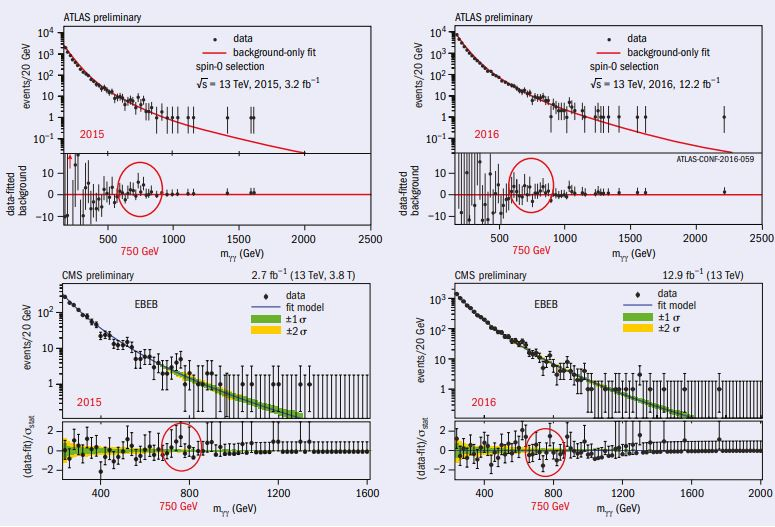
\includegraphics{figure_1A.JPG}
\caption{title}
\end{figure}

\begin{quote}
In a dramatic parallel session, both ATLAS and CMS revealed that their
2016 data do not confirm the previous hints of a diphoton resonance at
750 GeV (figure 1); apparently, those hints were nothing more than
tantalising statistical fluctuations.
\end{quote}

    \hypertarget{i-write-two-sentences-explaining-what-the-look-elsewhere-effect-is.}{%
\subsubsection{(i) Write two sentences explaining what the
`look-elsewhere effect'
is.}\label{i-write-two-sentences-explaining-what-the-look-elsewhere-effect-is.}}

    YOUR ANSWER HERE

    \hypertarget{ii-there-are-typically-more-than-100-papers-a-year-from-these-detectors-each-of-which-has-up-to-10-histograms-each-of-which-has-50-100-bins.-assuming-that-there-are-105-bins-in-a-year-how-many-2-3-4-and-5sigma-events-will-there-be}{%
\subsubsection{\texorpdfstring{(ii) There are typically more than 100
papers a year from these detectors, each of which has up to 10
histograms, each of which has 50-100 bins. Assuming that there are
\(10^5\) bins in a year, how many 2, 3, 4 and 5\(\sigma\) events will
there
be?}{(ii) There are typically more than 100 papers a year from these detectors, each of which has up to 10 histograms, each of which has 50-100 bins. Assuming that there are 10\^{}5 bins in a year, how many 2, 3, 4 and 5\textbackslash{}sigma events will there be?}}\label{ii-there-are-typically-more-than-100-papers-a-year-from-these-detectors-each-of-which-has-up-to-10-histograms-each-of-which-has-50-100-bins.-assuming-that-there-are-105-bins-in-a-year-how-many-2-3-4-and-5sigma-events-will-there-be}}

    \begin{Verbatim}[commandchars=\\\{\}]
{\color{incolor}In [{\color{incolor} }]:} \PY{k}{def} \PY{n+nf}{six\PYZus{}ii}\PY{p}{(}\PY{p}{)}\PY{p}{:}
            \PY{l+s+sd}{\PYZsq{}\PYZsq{}\PYZsq{}Your function should return the number of 2,3,4,5 sigma events\PYZsq{}\PYZsq{}\PYZsq{}}
            \PY{c+c1}{\PYZsh{} YOUR CODE HERE}
            \PY{k}{return}\PY{p}{(}\PY{n}{two\PYZus{}sigma}\PY{p}{,} \PY{n}{three\PYZus{}sigma}\PY{p}{,} \PY{n}{four\PYZus{}sigma}\PY{p}{,} \PY{n}{five\PYZus{}sigma}\PY{p}{)}
\end{Verbatim}


    \hypertarget{iii-what-are-the-chances-of-two-2sigma-events-at-the-same-energy}{%
\subsubsection{\texorpdfstring{(iii) What are the chances of two
2\(\sigma\) events at the same
energy?}{(iii) What are the chances of two 2\textbackslash{}sigma events at the same energy?}}\label{iii-what-are-the-chances-of-two-2sigma-events-at-the-same-energy}}

    \begin{Verbatim}[commandchars=\\\{\}]
{\color{incolor}In [{\color{incolor} }]:} \PY{k}{def} \PY{n+nf}{six\PYZus{}iii}\PY{p}{(}\PY{p}{)}\PY{p}{:}
            \PY{l+s+sd}{\PYZsq{}\PYZsq{}\PYZsq{}Your function should return the probability of two 2 sigma events at the same energy\PYZsq{}\PYZsq{}\PYZsq{}}
            \PY{c+c1}{\PYZsh{} YOUR CODE HERE}
\end{Verbatim}


    \hypertarget{coding-exercise}{%
\subsection{Coding Exercise}\label{coding-exercise}}

Choose one of the distributions we discussed in the context of the
Central Limit theorem: either the uniform distribution, the triangular
distribution or a Gaussian distribution. They should span the interval 0
to 1. Write code that allows you to choose numbers at random from this
distribution. Then,

 (i) Choose 1,000 numbers at random, and plot a histogram of their
occurrences.

\begin{enumerate}
\def\labelenumi{(\roman{enumi})}
\setcounter{enumi}{1}
\tightlist
\item
  Choose 2 numbers from the distribution at random, and average them.
  Repeat this 1,000 times and plot a histogram. 
\end{enumerate}

\begin{enumerate}
\def\labelenumi{(\roman{enumi})}
\setcounter{enumi}{2}
\tightlist
\item
  Do the same for the sum of 3, 4 and 5 numbers, and make the
  corresponding plots. 
\end{enumerate}

\begin{enumerate}
\def\labelenumi{(\roman{enumi})}
\setcounter{enumi}{3}
\tightlist
\item
  Comment on your results.
\end{enumerate}

    \begin{Verbatim}[commandchars=\\\{\}]
{\color{incolor}In [{\color{incolor} }]:} \PY{c+c1}{\PYZsh{} YOUR CODE HERE}
\end{Verbatim}


    \hypertarget{iv-comment-on-your-results.}{%
\subsubsection{(iv) Comment on your
results.}\label{iv-comment-on-your-results.}}

    YOUR ANSWER HERE


    % Add a bibliography block to the postdoc
    
    
    
    \end{document}
